
\documentclass[twocolumn]{article}
% {amsart}
\usepackage[top=0.75in, left=0.65in, right=0.65in, bottom=0.6in]{geometry}

\usepackage{float}

% \usepackage{url}
% \usepackage{xurl}
\usepackage[pdftex]{hyperref}

% code sux, use "lstlisting"
%\usepackage{code}
\usepackage{listings}
% \usepackage{cite}
\usepackage{latexsym}
\usepackage{amsmath}
\usepackage{amssymb}
\usepackage{graphicx}
% IPA symbols. safe turns off overrides for like \! which I still want
% \usepackage[safe]{tipa}
% \usepackage{chessboard}
% \usepackage{supertabular}
\usepackage{enumitem}

% \usepackage[most]{tcolorbox}

% lets me explicitly set a. or 1. etc. as enum label
% \usepackage{enumitem}

\pagestyle{empty}

\usepackage{ulem}
% go back to italics for emphasis, though
\normalem

% do "fancy" stuff like verbatim in footnotes
\usepackage{fancyvrb}
\VerbatimFootnotes

\usepackage{natbib}
\setcitestyle{numbers,square}

\interfootnotelinepenalty=0
\setlength{\footnotesep}{2em}

% \startsquarepar and \stopsquarepar allows justifying the
% whole paragraph, including its last line
\newcommand{\startsquarepar}{%
    \par\begingroup \parfillskip 0pt \relax}
\newcommand{\stopsquarepar}{%
    \par\endgroup}

% Style for code listings.
\lstdefinestyle{codestyle}{
  basicstyle=\ttfamily\footnotesize,
  breaklines=false,
  keepspaces=true,
}

\lstset{style=codestyle}

\newcommand\sfrac[2]{\!{}\,^{#1}\!/{}\!_{#2}}
\newcommand\xbyx[2]{\ensuremath{#1 {\times} #2}}


% XXX the collection of crap above causes a first page
% with just "1" on it (probably conflicting packages). This
% magic just drops the first page, which is of course not
% the right solution, but...

\usepackage{atbegshi}% http://ctan.org/pkg/atbegshi
\AtBeginDocument{\AtBeginShipoutNext{\AtBeginShipoutDiscard}}

\begin{document}

\title{GradIEEEnt half decent}
\author{Dr.~Tom~Murphy~VII~Ph.D.}\thanks{
Copyright \copyright\ 2023 the Regents of the Wikiplia Foundation.
Appears in SIGBOVIK~2023 with the
signaling NaN
of the Association for Computational Heresy; {\em IEEEEEE!}
press, Verlag-Verlag volume no.~0x40-2A. 1 ULP
}

\renewcommand\th{\ensuremath{{}^{\textrm{th}}}}
\newcommand\st{\ensuremath{{}^{\textrm{st}}}}
\newcommand\rd{\ensuremath{{}^{\textrm{rd}}}}
\newcommand\nd{\ensuremath{{}^{\textrm{nd}}}}

\newcommand\gradone{{\sf grad1}}
\newcommand\downshifttwo{{\sf downshift2}}
\newcommand\plussixtyfour{{\sf plus64}}

\renewcommand\paragraph[1]{\smallskip \noindent{\bf #1}\enspace}

\date{X April 2023}

\maketitle \thispagestyle{empty}

\sloppypar


\section{Introduction}



Imagine you are my professor. Maybe you actually were my professor, in
which case you may already be sweating before I say any more. The
subject matter is Neural Networks. You draw the

``Now this transfer function can be almost anything. Typically it
would be something like the hyperbolic tangent, which looks like this.

\begin{center}
\includegraphics[width=0.75 \linewidth]{tanh}
\end{center}

``But it has to be a non-linear function. If it's linear, i.e.~of the
form $y = mx + b$, then observe that the entire layer is a linear
function. And so the entire network is just a linear function of
linear functions; itself a linear function. We could just compute an
equivalent single-layer network, and we know that it could only fit
linear functions, which is insufficient for most problems.''

Then I raise my hand. The speed with which I raise it, and the subtle
forward pose of my arm suggests that I want to pluck an abstract idea
from the whiteboard and pervert it. You know this look, and you're
reluctant to call on me. But no other students are asking questions.
You must call on me.

``Tom.'' It's more like a statement then a question. It includes the
tone of spoken punctuation that, if it could, ends the entire
conversation before it begins.

``OK but, when we implement this on a computer we'll use some
approximation of numbers, like floating point. So the specific
sequence of additions and multiplications will matter. It's not
actually equivalent to rearrange them to a single layer because you
don't have distributivity, commutativity, etc.''

``Uh. I think that's technically true, but for all practical purposes \ldots''

``What about *im*practical purposes?''

You vigorously strangle me, and I die.

$\bigskip$
$\cdots$
$\bigskip$

That was about 20 years ago. The world will not let us stop thinking
about neural networks. And so this question has been on my mind for a
long time. Just to be clear, the professor was right: This is not an
important question. Theoretically I am right, but for practical
purposes it probably does not matter. But I like to work at the
intersection of Theory and Impractice. We can make it matter by doing
a lot of work. And then I will continue to be right theoretically, but
also more right because it will only matter for {\em most} practical
purposes.

So this paper is an exhaustive exploration of what we can do with just
floating point addition and multiplication by constants (scaling). You
should only be able to make lines, but I'll demonstrate that due to
rounding error, you can absolutely use ``linear'' transfer functions
in neural networks. Machine learning is not the only field with a
proclamation that some function must be ``non-linear,'' so we'll look
at a few of those as well. There will of course be several hearty
digressions. By studying these functions we'll see that they are
almost arbitrarily rich, and conclude with a demonstration of their
completeness in the field of Plumbing.

TODO intro: We'll develop a better understanding of where floating point inaccuracy comes from, and how to get it quickly, and how to use it for our benefit.

\section{A Refresher on Neural Networks}
Let's repeat the professor's lesson. This section is easily skippable
if you are a plucky student who thinks they already know everything.
At a high level, a NN is a way of implementing a numeric function
(takes a bunch of numbers as input, and gives a bunch of numbers as
output). The network consists of a number of {\it layers}, where the first
layer is the input and the last layer is the output.

TODO DIAGRAM

The numbers that fill in each layer are its {\it activations}. Each
layer's activations are computed from (just) the previous layer,
according to a formula:

$$a_i = TF(w_{1i} * p_1 + \ldots w_{ni} * p_n + b_i)$$

Where $p_j$ is the activation of the $j$th node on the previous layer,
and $w_{ji}$ is the weight parameter, and $b_i$ is the bias parameter.
The weight and bias parameters are learned during the training of the
neural network, but just become constants when using the NN to compute
its output.

$TF$ is the transfer function, which is of particular interest in this
project. Classically, the transfer function was some kind of sigmoid.
The {\tt tanh} function pictured in the introduction is a good example
of a sigmoid. The intuition behind this is that, thinking about $a_i$
as some kind of neuron, the neuron ``fires'' (activates) with some
probability. This probability gets higher as its input values get
larger (but note that weights can be negative, so upstream neurons can
also have an inhibitory effect). But since it is a probability, the
value must be in [0, 1]; the transfer function ensures this.

\paragraph{Differentiability.}
Another important property of the transfer function is that it be
differentiable, because the stochastic gradient descent algorithm used
to train NNs needs to be able to move along some error-reducing
gradient, and back-propagate errors to earlier layers. This gradient
is just the derivative of the function.

\paragraph{What transfer functions ought to exist?}
We used to think that these saturating transfer functions were ideal.
But this turns out to be wrong, especially for internal (``hidden'')
layers. Transfer functions don't need to produce probabilities, and
they can have unbounded range. A wide variety of functions will work,
including extremely simple ones. The most popular transfer function in
2023 is the ``rectified linear unit,'' which looks like this:

\begin{center}
\includegraphics[width=0.33 \linewidth]{relu}
\end{center}

This one is extremely easy to implement (\verb+x < 0 ? 0 : x+), is fast
and seems to work very well, possibly because its derivative is
significant (one) on the entire positive side. (In contrast, sigmoids
tend to get ``stuck'' because of their saturating behavior; their
derivatives become nearly zero.) Note that it is not actually
differentiable (discontinuity at zero) but ``for all practical
purposes'' it is differentiable.

The (only?) apparently essential quality of the transfer function is
that it be non-linear. If it is instead of the form $TF(x) = mx + b$,
then $a_i$ is also just a linear function of the previous layer, as
linear functions of linear functions (weighted sum) are linear. This
causes the entire NN to be a linear function. It is well known that a
linear function ``cannot'' represent some other simple functions, such
as XOR.

$$\nexists m,n,b.\,\, XOR(x, y) \approxeq m x + n y + b$$
% FORMULA: Not exists m n b, such that $XOR(x, y) \approxeq m x + n y + b$

This means that with a linear transfer function, a NN could never
learn even a simple function like XOR. Many problems we want to learn
are in fact much more complicated.

\section{A Fine Terminological Issue}
affine vs linear

(Here we need to clarify exactly what operations we allow!) THE RULES


\section{Half-precision IEEE-754 floating point}
In this project we'll abuse floating point inaccuracy to create
``linear'' functions (only using floating point addition and scaling)
that are not lines. For this reason, we prefer to have a numerical
system that is {\em less accurate}. In floating point, inaccuracy comes
from the fact that not all numbers are representable (due to finite
precision) and the result of an operation is always rounded to a
representable number. IEEE-754 floating point comes in different
``spice levels,'' with ``32-bits'' being ``float'' and ``64-bits''
being ``double.'' Although spice levels as low as 3 bits make
sense\cite{murphy2019nan}, 8-bit (``mild'') is occasionally used in
real applications, and 16-bit (``half'') is quite common in machine
learning. Usually the reason to prefer half precision is that it uses
less memory, and so your GPU can store networks that are twice as big
in RAM. For this project we will also use half precision, and we will
be happy to save RAM, but more happy that its precision is low and so
it is practical (although silly) to achieve significant rounding
error. Another important reason to choose half precision is to make
the pun in the title.

A half precision float is 16 bits: One sign bit, five bits for the
exponent, and 10 bits for the mantissa. Like all IEEE-754 formats,
there is much more precision (more values are representable) near
zero. (Figure~\ref{fig:histogram}) Once you get to 1024,
only integers are representable. From 2048 to 4096, only even numbers
are representable. 65504 is the largest finite number, and up here,
only multiples of 32 are available.

\begin{figure}
FIGURE: HISTOGRAM
\caption{
Here I will put a histogram of the values.
  } \label{fig:histogram}
\end{figure}

% Where does floating point imprecision come from?
\paragraph{Origins of Imprecision.}
Floating point does have many perversions, but many programmers come
to believe all sorts of dangerous superstitions about it. One idea is
that floating point is somehow always inexact, and so that you always
have to check that two numbers are equal ``within some
epsilon''\cite{murphy2014epsilon}. This may work ``in practice'' but
it is actually pretty sloppy. Floating point imprecision is not
random, nor is it constrained to a fixed epsilon. Operations are
defined much more usefully: Each one computes the mathematically
correct value, and then rounds (according to the ``rounding mode'') to
the nearest representable value. That's it. One consequence of this is
that you can get the exact result of 32-bit multiplication by doing
64-bit multiplication and then rounding to 32 bits. This also means
that the rounding error from a single operation can be as large as the
gap between representable numbers: Up to 32 for half-precision. But it
also means that operations whose results can be exactly represented
have no error; for example adding integral half values less than 512
will always give an exact integer result, which can be compared using
==. We will use this later in Section~\ref{sec:sixtyfive}. It is
neither necessary nor sufficient compare for ``equality'' with some
``epsilon.''

\paragraph{Rounding.}
IEEE-754 supports multiple rounding modes, like ``round-to-zero,'' and
``round-to-infinity'' (always round in the positive direction).
Throughout this paper we use ``round-to-nearest,'' which is also the
typical default (e.g.~for C++11 expressions evaluated at compile time,
it always uses round-to-nearest).\footnote{There is seldom reason to
  change the rounding mode, and since it is a stateful act, you're
  asking for it if you do. But the round-to-negative-infinity and
  round-to-positive-infinity modes are are useful for interval
  arithmetic, which is arguably the only truly reasonable way to use
  floating point. What you do is represent numbers as intervals (low
  and high endpoints) that contain the true value, and then perform
  each calculation on both endpoints. For computations on the low
  endpoint, you round down, and symmetrically for the high endpoint.
  This way, the true value is always within the interval, and you also
  know how much inaccuracy you have accumulated!} Similar results are
likely attainable for the other rounding modes, as well as
hypothetical rounding modes such as ``round away from nearest,'' but I
have not explored this.

\paragraph{Getting some nonlinearity.}
All transfer functions implemented with floating point have a finite
range. For our experiments with neural networks, we will focus on
transfer functions that map values in [-1, 1] to values in [-1, 1].
Almost half (48.4\%) of floating point values are in this interval and this
is a typical nominal range for activations in neural networks.

We only have two operations: Addition and scaling. Let's see what kind
of rounding error each of these gives us. First, addition. In order to
get a function that takes values in [-1, 1] to values in [-1, 1], we
want to first add a constant (giving us perhaps a large value) and
then add a negative constant, bringing us back in range. For example,
the constant 128 gives us the function

$$f(x) = x + 128.0 - 128.0$$

This is of course mathematically the same as $f(x) = x$ (the
identity), but with half precision we get a function that looks like
this

\begin{center}
\includegraphics[width=0.45 \linewidth]{plus128}
\end{center}


Between 128 and 256, only multiples of 0.125 are representable. So for
arguments in 0 to 1, the sum is rounded to one of the values 128.0,
128.125, 128.25, \ldots 129. From 64 to 128, multiples of .0625
($\sfrac{1}{16}\th$) are representable. So from -1 to 0, we get 127.0, 127.0625,
127.125, \ldots 128. Subtracting 128, all of the values are exactly
representable, giving us -1, -.9375, \ldots, -0.0625, 0, 0.125,
\ldots, 0.875, 1.

The result is a step function, but whose resolution is twice as high
for the negative range as the positive; had we added -128 and then
added 128, we would have seen the opposite bias in resolution. We can
easily see that this function is (computationally) ``non-linear''
despite being (mathematically) ``linear.'' This function is unlikely
to be a good transfer function, because it does not have a good
derivative: It's zero most places (flat segments) except at the
discontinuities, where it is undefined. We do test this approach
(with the constant 64.0) later, though.

Scaling gives similar results. Consider

$$f(x) = x * 100.0 * (1.0 / 100.0)$$

In this project we never actually divide (although this would not
violate linearity) since most floating point numbers have approximate
multiplicative inverses, and many are exact. We just compute the
reciprocal $\sfrac{1}{100} \approxeq 0.01000213623$ ahead of time and
multiply by that constant. Here's what that function looks like:

\begin{center}
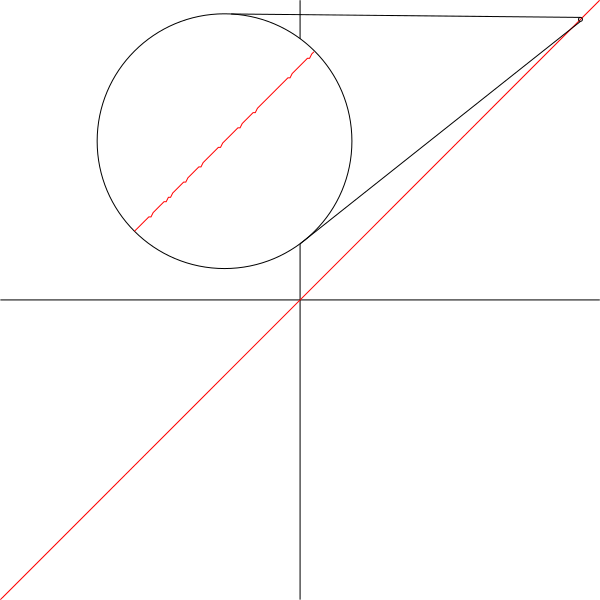
\includegraphics[width=0.45 \linewidth]{times100zoom}
\end{center}

At this scale it appears linear, but it does have small imperfections
(see zoomed region). The function is symmetric about zero, since
multiplication will do the same thing to a positive number as it does
to its negative counterpart. Here, the roundoff error differs with the
magnitude. At inputs close to 1.0, the results of the first
multiplication must round to the nearest multiple of 0.0625 (as in the
additive example) but this error is scaled down by a factor of 100
when we multiply back to the [-1, 1] range. So it is almost invisible.
For inputs close to 0.0, the error approaches zero. The effect is complex
and depends on the constant we multiply by. For example, if we multiply
by a power of two, this only affects the exponent, and so the result is
exact.

\medskip
Is that it? Of course not! We can apply these operations in
combination, and many times, to create more interesting functions. The
best approach I found in this simple family is to repeatedly multiply
the input by a number very close to one. Here's what happens if you
multiply the input by $0.99951171875$ (which is the next number
smaller than one, equal to $1 - \sfrac{1}{2048}$) five hundred times,
and then scale back at the end:

\[
\begin{array}{rcl}
  f(x) & = & x * (1 - \sfrac{1}{2048}) * (1 - \sfrac{1}{2048}) * \ldots \textrm{500 times} \ldots * \\
  \, & \, & 1.3232421875$$
\end{array}
\]

\begin{center}
\includegraphics[width=0.85 \linewidth]{grad1}
\end{center}

I call this the \gradone\ function.

Multiplying $1.0$ by $(1 - \sfrac{1}{2048})$ five hundred times in
half precision yields $0.755859375$ (mathematically it would be $(1 -
\sfrac{1}{2048})^{500} = 0.78333$, so there is significant accumulated
error. We set $f(1.0) = 1.0$ by multiplying by the inverse of this
constant, which is $1.3232421875$.

Why does this result in the zig-zags? Multiplication by $(1 -
\sfrac{1}{2048})$ affects numbers differently. For constants less than
$6.1094760895 \times 10^{-5}$, the value is unchanged; we round back up to
the original value. For all other finite inputs it produces a smaller
value, but with rounding error that depends on the value. This error
accumulates and becomes significant with many iterations
(Figure~\ref{fig:rainbow}). Unlike the previous functions, the output
here is much smoother (it looks piecewise-linear); in each of these
segments its derivative is nondegenerate. Of course, this function is
mathematically linear. It is equivalent to $f(x) = x * 1.036535$.

\begin{figure}[htp]
  
\includegraphics[width=0.95 \linewidth]{rainbow} \\[1em]
  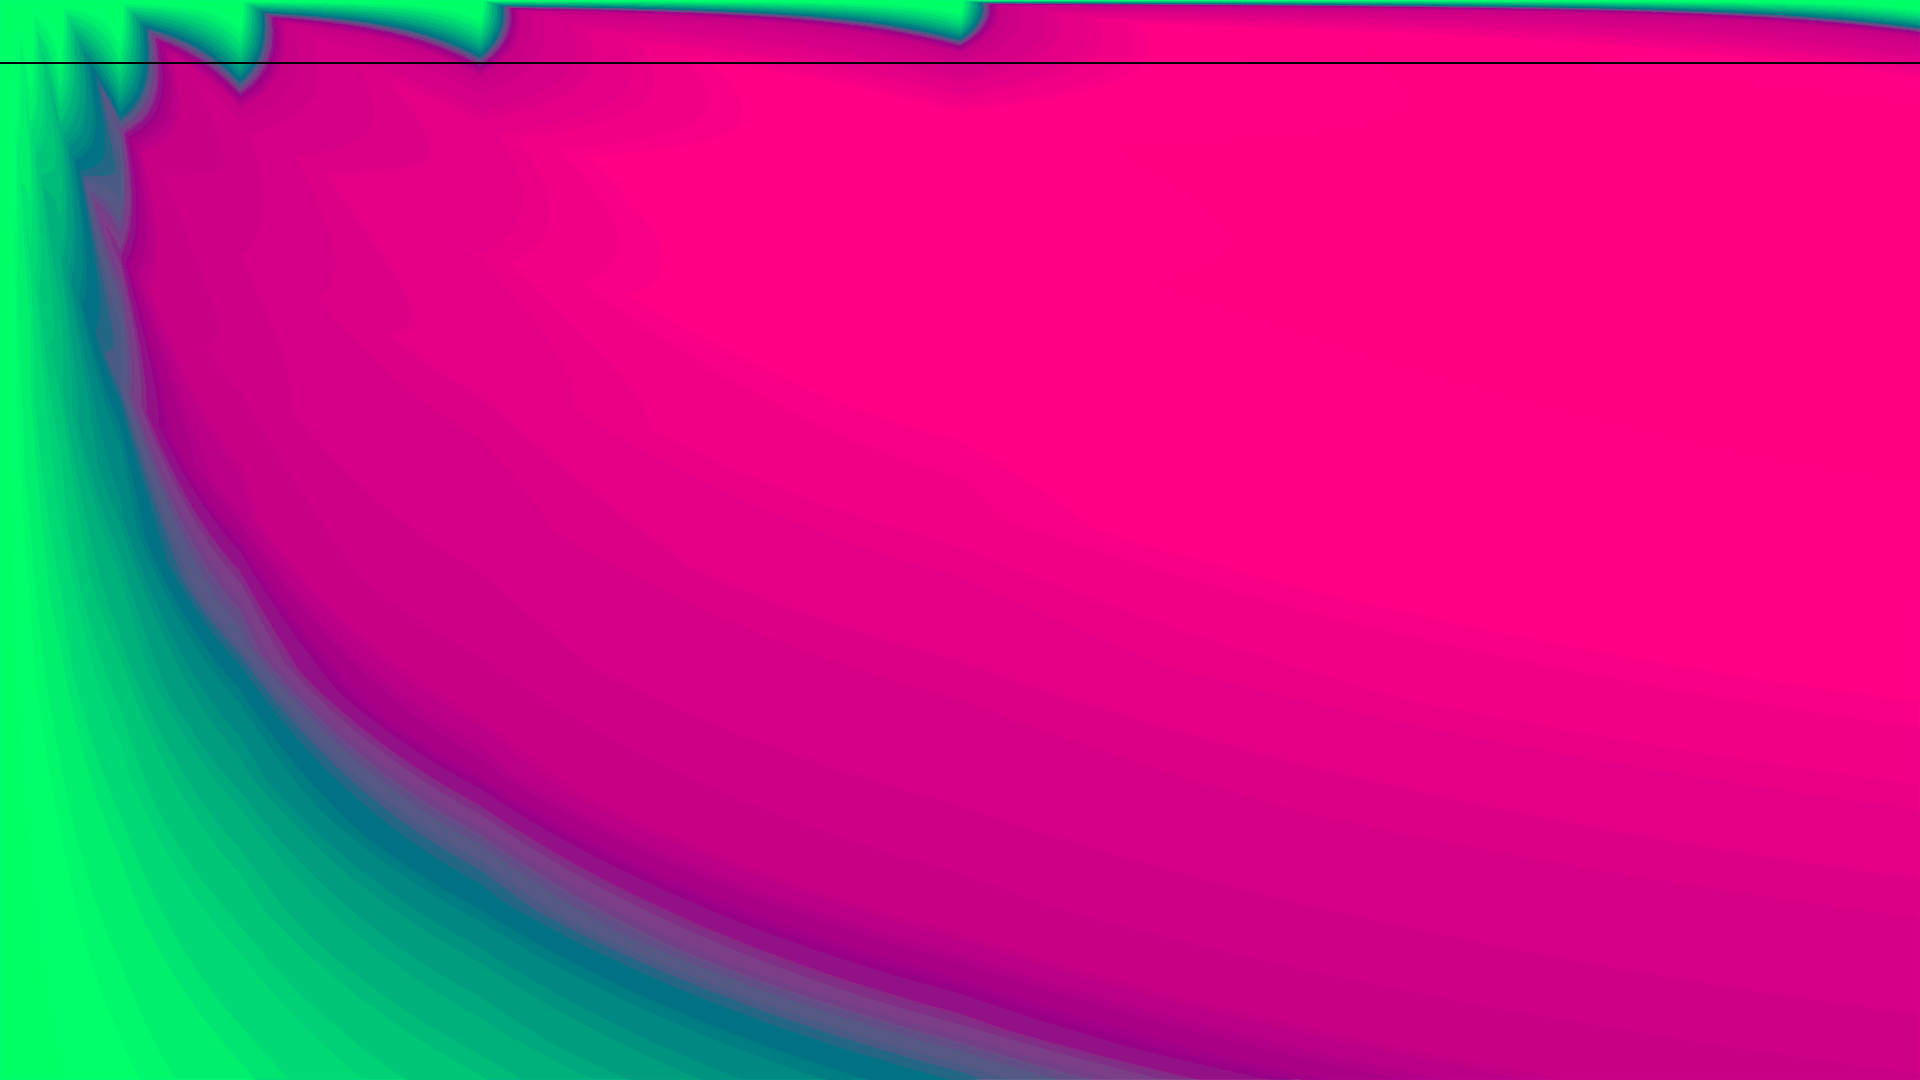
\includegraphics[width=0.95 \linewidth]{rainbow-error}
  \caption{
    How repeated multiplying by $1 - \sfrac{1}{2048}$ affects values in
    [0, 1].
    The width of the image is the interval [0, 1], with zero at the left.
    \\[1em]
    {\bf Top}: In the topmost row, we assign each pixel a hue so that
    we can track where those values go. For each pixel, we
    successively multiply by the constant and plot its color in its
    new $x$ position, the move to the next row down. Note that the
    rainbow shrinks exponentially as expected, but not smoothly.
    The black line is 500 iterations.
    \\[1em]
    {\bf Bottom}: The accumulated error when iteratively multiplying
    by the constant. Here the $x$ coordinate of the value does not move
    (so the middle column always represents the value that was
    originally 0.5). The color illustrates the accumulated error. For
    green pixels, the value is too high compared to the mathematically
    correct one; for magenta pixels too low. By choosing a row with
    alternations between green and red, we get the zig-zag pattern of
    the \gradone\ transfer function.
  } \label{fig:rainbow}
\end{figure}

% XXX DELETE Another nice thing about this function is that it does not introduce unnecessary infinities. The previous functions both overflow on some inputs. For example, adding 128 to the largest finite value 65504 (and several values smaller than that) gives inf, from which there is no way back. In contrast, multiplying by a number slightly less than one never in (XXX is this true because of the last scaling?) (XXX No it is not!)

So now we have a ``good'' candidate function, which we'll call \gradone.
It is ``good'' in the sense that it is computationally non-linear
despite being mathematically linear, so it may prove my professor
wrong. On the other hand, it requires 501 floating point
multiplications to compute, which is kind of slow. The ``good'' news
is that since there are only 65536 16-bit values, we can easily just
precompute any function for all possible half inputs, and store it in
a table of 131072 bytes. This allows us to execute the function
efficiently when performance is important, such as during training.
(Table lookup is certainly not a mathematically linear operation, so
when we require the computation to be linear for ideological purposes,
we can perform the 501 multiplications and get the same result.)

\paragraph{Differentiating.}
Speaking of training, in order to train a neural network using
stochastic gradient descent, we need to be able to evaluate the
derivative of the transfer function at any point.
 XXX TODO EXPLAIN IT

\subsection{Bonus Digression}
Having freed myself from needing to ``do math'' in order to
differentiate exotic functions, I pondered other weird transfer
functions. For example, the rectified linear transfer function is very
simple and works well, but is it the fastest possible transfer
function that might work? It does involve a conditional, which naively
implies comparison and branching (although probably most processors
can do this with a conditional move). Because the floating point
format is packed with fields that represent different things, many
simple operations on its bits have interesting non-linear behavior.
The most promising I found was a right shift by two places.

\begin{center}
\includegraphics[width=0.95 \linewidth]{downshift2}
\end{center}

TODO: Diagrams of other operations

Shifting is about the cheapest possible thing a processor can do. Its behavior on floating point numbers is interesting,

DIAGRAM: TODO: in illustrator

\begin{verbatim}
[s][e][e][e][e][e][m][m][m] [m] [m] [m] [m] [m] [m] [m]
[0][0][s][e][e][e][e][m] [m] [m] [m] [m] [m] [m] [m]
\end{verbatim}

The sign bit is shifted into the exponent, which means that the output is always non-negative (like the rectified linear function) and is non-linear (discontinuity at zero, as negative numbers have a much larger exponent that positive ones). Further nonlinearity comes from the exponential representation (shifts divide the exponent by four) and reinterpretation of exponent bits as mantissa bits. There is additional weirdness in the details. Shifting by two places is better than one, as it cannot produce Inf or NaN. We will also evaluate this transfer function, called shift2, below.

I implemented all this as a modification of my custom NN training and inference system, ``Tom7Flow.'' Tom7Flow is generally much worse than mainstream packages; it is based on deprecated OpenCL technology, is prone to divergence or stagnation during training due to naive choices of hyperparameters, etc. But it is at least well suited to silly experiments that take the form, ``What if deep learning but worse?'' such as the current exercise. In order to realize the idea completely, I modified the inference code to calculate with half-precision arithmetic (not just the transfer function). This means that the trained networks can be executed using only half-precision operations (and just addition and multiplication by constants). Unfortunately, while my GPU supports half-precision math natively, and OpenCL supports half-precision operations as an extension, this extension is somehow not supported (??) by my drivers, perhaps because OpenCL is so thoroughly deprecated. It does support half precision as a *storage* format, which allows you to write a full-precision float to a 16-bit value (rounding to half) or read a 16-bit half into a float (all half values can be represented exactly in full precision). So with this one operation it is straightforward to implement half-precision addition and scaling. You maintain the invariant that any float value is always exactly a half, and after you perform addition or multiplication, you round to half (by storing in a 16-bit memory location and reading it back). This definitionally produces the same results as the native operation.

I initially tried a version of training that worked entirely using
half precision (network parameters are half, backpropagated errors and
update values are half, etc.). This worked badly. It is ideologically
unnecessary, as we just care about producing a final model that,
during inference, only executes linear half-precision operations (but
abuses floating point roundoff to do something interesting.) This
network can be trained using non-linear techniques (and must anyway,
since for example its computed derivative is not linear). So during
training, calculations are done using full-precision floats, except
for the forward step (where we round to half after every operation).
In addition to being simpler, representing intermediate learned
weights as floats seems to help training approach the final half
values smoothly, avoiding stalls due to underflow.

TODO: half.h~\cite{half} somewhere above?

\subsection{Neural network experimental results}
In order to evaluate this transfer function, I ran a suite of benchmark problems. For each problem, I compare the same network architecture (i.e.~the number of layers, their connectivity, etc.) but using different transfer functions.

The transfer functions are:

\begin{itemize}
\item {\bf grad1}: The ``linear'' transfer function \gradone\ described above.
\item {\bf tanh}: The hyperbolic tangent function, which is a classic saturating (output is always in (-1, 1)) sigmoid.
\item {\bf logistic}: The function $1 / (1 + e^{-x})$, another classic sigmoid (but whose output is in (0, 1)). Each operation is performed with half precision.
\item {\bf leaky relu}: The rectified linear unit, but with a small slope below zero: \verb|x < 0.0 ? 0.1 * x : x|. This is the function I usually prefer in practice; its advantage over the standard relu is that it does not ``die'' (zero propagated error) when its input is negative.
\item {\bf downshift2}: Interpreting the half-precision input as a 16-bit word, right shift by 2 places, then reinterpret as half.
\item {\bf plus64}: $f(x) = x + 64 - 64$. This about the simplest function that has obvious rounding error. It only outputs 25 distinct values in [-1, 1] so its derivative is degenerate; I use its ``mathematical'' derivative $f'(x) = 1$.\footnote{Learning with this function might work better if we instead approximate the derivative by something non-constant, like by computing the derivative of a smoothed version. However, due to implementation tricks in Tom7Flow, we need a derivative that is expressed in terms of the transfer function's {\it output} (i.e.~$g(f(x))$ = $f'(x)$); we would not be able to express the smoothed derivative because there are only 25 distinct values of $f(x)$ in the [-1,1] range!}
\item {\bf identity}: The function $f(x) = x$. This is an important comparison because it shows us what a ``true'' linear (both mathematically and computationally) network is capable of.
\end{itemize}

TODO: Describe derivatives above?

\paragraph{MNIST.}
The first problem is the Modified National Institute of Standards and
Technology handwriting dataset (MNIST). This is a standardized dataset
of handwritten digits (0–9) as \xbyx{28}{28} greyscale images. This is chosen
partly for trollish reasons. It dates from 1998, and even at the time
of publication, accuracy with neural networks (98.4\%) and other
techniques (99.2\%) were already extremely high~\cite{lecun1998gradient}.

For this problem, I augmented the dataset by randomly offsetting the
training images by up to two pixels in any direction, and by adding
Gaussian noise. The model's input layer is just the $28 \times 28$
greyscale values, and the output is a prediction for each of the ten
digits. The models had two convolutional layers (64 \xbyx{3}{3} features,
fully overlapping + 128 \xbyx{8}{8} features, fully overlapping; then
32 \xbyx{128}{128} features + 32 \xbyx{256}{2} features with no
overlap), then two sparse layers of 1024 nodes each, then a final
dense output layer. The same initial weights and connectivity was used
for each experiment. Internal layers use the transfer function being
evaluated, but the output layer always used the identity transfer
function. This is not a good choice for this problem (softmax makes
more sense since the output is categorical) but I wanted the linear
models to be truly linear. Using the same transfer function would have
also disadvantaged functions with limited output range; \downshifttwo
for example can technically output 1.0, but only for very large inputs
(8192.0). The final identity layer can easily scale the useful range
of the transfer function to the nominal range of the output. (This is
essential for the chess problem below, where the output instead ranges
[-1, 1].)

See the source code for various hyperparameter settings (although if
you are trying to learn good settings for hyperparameters, my code is
not the place to look). I used the ADAM weight update
trick~\cite{kingma2014adam}, which does give me much better results
than plain SGD in my experiments.

\begin{figure}[htp]
  \begin{tabular}{rr}
{\bf transfer function} & {\bf accuracy} \\
\hline 
sigmoid & 98.20\% \\
tanh & 98.93\% \\
leaky-relu & 99.39\% \\
plus64 & 82.66\% \\
grad1 & 97.29\% \\
identity & 81.96\% \\
downshift2 & 94.45\% \\
\end{tabular}

  \caption{
    Results on the standardized MNIST data set. Accuracy is the
    fraction of results from the held-out test data for which the
    highest-scoring class (digit) is the correct class.
  } \label{fig:mnistresults}
\end{figure}

\begin{figure}[htp]
  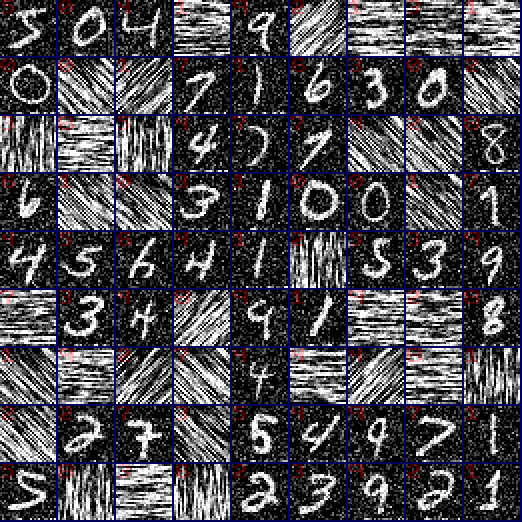
\includegraphics[width=0.9 \linewidth]{mnist-bug}
  \caption{
    Bug.
  } \label{fig:mnistbug}
\end{figure}

Results for MNIST are in Figure~\ref{fig:mnistresults}.
A nice bug appears in Figure~\ref{fig:mnistbug}.

\paragraph{CIFAR-10.}
Another classic dataset comes from the Canadian Institute For Advanced
Research. They capitalize ``For'' so that the acronym can be
pronounced nicely. I mean to be fair MNIOSAT would have a certain ring
to it too. This dataset contains 60,000 RGB images of size $32 \times 32$, that
are labeled into 10 classes: Airplanes, cars, birds, cats, deer, dogs,
frogs, horses, ships, and trucks~\cite{krizhevsky2009learning}. It is
very similar to the handwriting problem but more challenging (state of
the art accuracy is more like 96.5\%). Like with MNIST, I augmented the
training set by randomly shifting the images and adding Gaussian
noise. The network structure is the same as in the MNIST problem,
except that in the first convolutional layer, each window is three
times as wide to account for the three color channels.

\begin{figure}[htp]
  \begin{tabular}{rcr}
{\bf transfer function} & {\bf flat} & {\bf accuracy} \\
\hline
sigmoid &   & 56.83\% \\
tanh &   & 67.82\% \\
leaky-relu &   & 73.11\% \\
plus64 &   & 43.60\% \\
grad1 &   & 53.56\% \\
identity &   & 41.07\% \\
downshift2 &   & 46.54\% \\
plus64 & $\times$ & 32.76\% \\
grad1 & $\times$ & 30.58\% \\
identity & $\times$ & 41.04\% \\
\end{tabular}

  \caption{
    Results on the standardized CIFAR10 data set. As with MNIST,
    accuracy is the fraction of results from the held-out test
    data for whom the highest-scoring class is the correct class.
  } \label{fig:cifar10results}
\end{figure}


Results for CIFAR-10 appear in Figure~\ref{fig:cifar10results}.

\paragraph{Chess.}
This problem attempts to learn a good evaluation function for chess
boards. Training examples are real chess positions (from the Lichess
database) evaluated by a strong chess engine
(Stockfish~\cite{stockfish}). Stockfish generates two classes of
scores: ``Mate in N'' if one side is known to have a series of N moves
that wins (but ``Mate in 1'' is still better than ``Mate in 4''), or a
more subjective score, measured in pawns. (The score in pawns can
seemingly be arbitrarily high, which is kind of funny because how
could you even have that many pawns on a 64-square board? Here's an
idea for a SIGBOVIK paper: What's the highest scoring chess position,
according to Stockfish, for which it cannot deduce mate?)
% r1r1r2k/p1p1p1p1/PpPpPpPp/1P1P1P1P/BRBRBRBR/RBRBRBRB/BRBRBRBR/K1RBRBRQ w - - 0 1
% Evaluated as +99.0 at depth 56/99
Mate is of
course categorically better than the pawn score, as it is exact.
Anyway, I squash this score into the range [-1, 1] and that becomes
the training instance. This network's first layer has 256 \xbyx{3}{3}
convolutional features, overlapping, as well as 32 \xbyx{1}{1} and
128 \xbyx{8}{1} and \xbyx{1}{8}. Each of these is measured in terms
of squares on the board, but each square actually corresponds to 13
inputs, for the 13 possible things that can be in that square (exactly
one set to 1.0). We also have some non-square inputs, like the
castling privileges and en passant state. So it's not just the
convolutional features but some sparse nodes too. And then we have
some more layers (you can check out the source code if you really care
about these details, which I doubt!) and then a final dense layer with
a single output using the identity transfer function as before. No
training data augmentation here, but I do normalize the board so that
it is always white to move.

For chess we can compute the accuracy, comparing to Stockfish as
ground truth (Figure~\ref{fig:chessresults}). We can also use the
evaluation function to play chess. These chess ``engines'' just look
at the possible legal moves and take the move that is most favorable,
using the learned evaluation function (no game tree search). Playing
against the best of these (``leaky'') it subjectively makes decent
moves most of the time and can even beat me playing casually. I
noticed that it had a lot of trouble ``sealing the deal'' in totally
winning positions (which is not unusual for engines that don't do
game-tree search or use endgame tables), but the problem was actually
more shallow: Due to a bug\footnote{ I used the annotations like
  \verb|[%eval #12]| that appear on moves for many games in the
  Lichess database. I didn't notice that they do not appear on a
  game-ending move like \verb+Qh4#+! This does sort of make sense
  because the eval scores would have to be \verb|[%eval #+0]| (``mate
  in 0'') or \verb|[%eval #-0]| (necessitating use of the floating
  point coprocessor) to express the winner, and there does not seem to
  be a clean way to express the definite value of stalemate. } in the
way training examples are gathered, the models were never exposed to
checkmate or stalemate positions! Since training takes several days
per function and the iron-fistedly punctilious SIGBOVIK deadlines were
imminent, there simply wasn't enough time to retrain them with access
to these positions. However, since mate is a mechanical fact of the
game (like what moves are legal) it seemed reasonable to fix this in
the engine itself: When considering all the legal moves to make, it
infinitely prefers a move that results in checkmate, and considers a
move resulting in stalemate to have score 0.0, and otherwise uses the
evaluation function. These ``fix'' versions of each engine perform
very significantly better, although they likely overestimate the
performance we'd get by actually fixing the model; there's no
guarantee that it would be able to accurately recognize mate, and the
fixed versions' greedy strategy of taking mate in 1 is always
advantageous.

These players compete against each other as well as the engines from
the Elo World project~\cite{murphy2019eloworld}, giving a sense of
their strength in an absolute scale (Figure~\ref{fig:elo}). The raw
versions perform reasonably; they all work better than a simple engine
like ``take the move that minimizes the number of moves the opponent
will have,'' (\verb+min_oppt_moves+). The fixed versions are much
better, as expected. The ``linear'' engine using the
\gradone\ transfer function, is competitive with the NES Chessmaster
engine, and outperforms a 50\% dilution of Stockfish. This is pretty
solid given that it is doing no explicit game tree search. In fact
(aside from the wrapper implementing the rules of chess and finding
the maximum eval score), it is only performing a fixed expression of
floating point addition and scaling! We could make this even more
ideologically pure using techniques from Section~\ref{sec:sixtyfive}.

\begin{figure}[htp]
  \begin{tabular}{rcrr}
{\bf transfer function} & {\bf flat} & {\bf loss} & {\bf accuracy} \\
\hline
sigmoid &   & 0.168 & 72.046\% \\
tanh &   & 0.117 & 78.527\% \\
leaky-relu &   & 0.118 & 78.172\% \\
plus64 &   & 0.162 & 75.406\% \\
grad1 &   & 0.111 & 78.924\% \\
identity &   & 0.161 & 75.975\% \\
downshift2 &   & 0.211 & 68.066\% \\
plus64 & $\times$ & 0.161 & 75.779\% \\
grad1 & $\times$ & 0.527 & 58.187\% \\
identity & $\times$ & 0.161 & 75.975\% \\
\end{tabular}

  \caption{
    Results of learning Stockfish's position evaluation function.
    Stockfish scores are normalized to a [-1, 1] scale, and loss
    here is the average (L1) distance between the predicted score
    and actual Stockfish score, on some 100,000 positions from
    games not in the training set. Accuracy is the percentage of
    predictions whose sign agreed with Stockfish (e.g.~they both
    agree the white player is winning).
  } \label{fig:chessresults}
\end{figure}

\begin{figure}[htp]
  TODO
  \caption{Here I will put the ELO WORLD results.}
  \label{fig:elo}
\end{figure}

XXX compare ``flattened'' linear model. it may be the case
that real models take advantage of roundoff nonlinearity?

\paragraph{What transfer function is best?}
The results on each of these problems are similar: The ``leaky
rectified'' transfer function is generally best or close to best.
The identity transfer function, which yields a simple linear model,
is generally worst or close to worst. The sigmoid functions are
all over the place. The experimental \downshifttwo\ function is
generally bad, perhaps because its output is strictly positive or
it has such a small dynamic range. The small amount of nonlinearity
introduced by \plussixtyfour\ does seem to give it a small edge
over the identity, but its lack of an interesting derivative and
the fact that it only produces a small number of output values seem
to be limiting. Importantly, the \gradone\ function---the
centerpiece of the first third of this paper---performs decently on
all problems. It clearly outperforms the linear models, despite
being ``linear.''

Having proved the professor wrong, we could stop there, but did huge
mathematical breakthroughs ever arise from taking the option to stop
there?!


\section{Non-monotonic functions}
Because of the way that addition and scaling are defined (do the real
mathematical operation, then round), they preserve monotonicity: If $x
\geq y$, then $f(x) \geq f(y)$. But this is only true if we limit the
form of the function to a series of additions and (positive) scaling.
There are other expressions that are mathematically linear but don't
take that form; for example:

$$f(x) = x + 0.25 - x$$

This is mathematically equivalent to $f(x) = 0.25$, but with floating point, it
is a boxcar function (CHECK)

% XXX this would instead be zigzags, right?
\begin{center}
\includegraphics[width=0.75 \linewidth]{boxcar25}
\end{center}

It takes the value 0.25 in places where there is enough precision to
represent $x + 0.25$, or 0 when $x + 0.25$ rounds to $x$.

Here is $f(x) = \gradone(x) - x$, which is also linear:
\begin{center}
\includegraphics[width=0.75 \linewidth]{grad1minusx}
\end{center}

Generally speaking, we can create a large variety of functions by
computing the interference patterns between other functions, since the
sum or difference of two ``linear'' functions is also ``linear.'' In
general we'll consider expressions of this form:

\[
\begin{array}{rrl}
E & ::= & x              \\
  &  |  & E * {\tt c}    \\
  &  |  & E + {\tt c}    \\
  &  |  & E + E          \\
\end{array}
\]

Where $x$ is the function variable, and {\tt c} is one of the 63,488
finite half-precision constants. We can derive negation $(E * -1)$ and
subtraction of constants $(E + -{\tt c})$ and expressions $(E + (E *
-1))$ since every number has an exact negation by flipping its sign
bit. Most divisions are also possible, when $\sfrac{1}{{\tt c}}$ is
representable.

(HERE, can we get an animation approximating the sine function or something?)

This formulation leads to a tempting approach for approximating a function iteratively, like a Taylor series. Given a target function like $sin(x)$, we can begin with an approximate expression for it, like $x$, and then add and subtract terms to improve the approximation. I don't know of any systematic way to improve the approximation at each step (they are not well-behaved mathematically, and I am not good at math), but by using computer search I can sure make some complicated functions with many different shapes.

It is fun to watch an animation of the successively improving approximations, but you can't see that since you're reading an old-fashioned paper. Perhaps you can find a video of this at tom7.org/grad.


OLD Given a target function $r$ like $r_0(x) = sin(x)$, we start with an approximation of it, like

$$f_1(x) = x$$

and then we have a new target function

$$r_1(x) = r_0(x) - f_1(x)$$

which is the residual error.


Next, I endeavored to deploy these functions for something useful: Fractals. Famously, fractals are simple functions with complex (often literally) behavior. For example, the Mandelbrot set considers each complex point $c$ (plotted on the plane as $x + yi$) and computes whether $z_i$ = $z_{i-1}^2 + c$ diverges or not. It's lovely, but squaring is not linear!



Bonus Digression: Baffling numbers


Drawing fractals is fun and everything, but I grew weary of the
exercise because there is no real goal other than to make a cool
picture. Instead I turned to something with a clearer challenge to
overcome: Linear Cryptography.

\section{Linear Cryptography}
Cryptography is like fractals minus drugs. One of the most basic
components of cryptography is a pseudorandom number generator. This
kind of function takes some state and produces a new state that
``looks random.'' Given a pseudorandom number generator, we can
construct one-way functions (``hash functions'') and from those we can
make symmetric ciphers (using, say, a Feistel network), with which we
can encrypt and decrypt data.

Another thing that professors will tell you about cryptography is that good cryptographic functions cannot be linear. (XXX an explanation of what ``linear'' means in this context. Like XOR is linear, but we used that as an example that has no linear approximation in the NN section.) One good reason for this is that even if the function is a *little bit linear* then linear cryptanalysis can be used to recover bits of the key with a lot of example data. Standard advice is to alternate both linear (e.g.~xor, or multiplication mod $2^n$) and non-linear (e.g.~substitution) operations. [[XXX citation here, like from Applied Cryptography.]] Of course we will prove this wrong by developing a good pseudorandom function that uses only ``linear'' operations on half-precision floating point numbers.

$\uparrow$ Here's a good description of linear cryptanalysis of DES: https://www.apprendre-en-ligne.net/crypto/bibliotheque/PDF/lincrypt.pdf

In terms of goals, pseudorandom number generation has a more clear objective than fractals, although it's not so easy to pin down formally. We don't even know if such functions exist, mathematically. (XXX cite) There exist many functions that look like good pseudorandom generators, but that actually have back doors that make them easy to invert. (A symmetric encryption algorithm like AES, with the key hidden, has this property.)\footnote{And let us never forget that RSA DSI (yes, that RSA) took a \$X million bribe from the NSA to put a backdoor in one of their pseudorandom number generators!} Practically speaking, though, we can subject the function to a wide variety of statistical tests, and if it looks random to every test, then this gives us good confidence.\footnote{Truly good cryptographic algorithms are also openly studied by experts. Of course nothing in here is to be used seriously, and not just because these algorithms are ridiculously slow!}

Specifically, my goal is to design an algorithm that takes 64 bits of data (represented as half-precision floats) to another 64 bits, such that the stream of low-order bits from iterating this function passes the TestU01's ``Big Crush'' suite of 106 statistical tests\cite{XXXbigcrush}. This suite is a successor to Marsaglia's ``DieHard'' battery of tests\cite{XXXmarsaglia}, itself an improvement on Knuth's tests from The Art Of Computer Programming\cite{XXXknuth}.

The basis of this function is the classic substitution-permutation network. First, each of the eight bytes are substituted with a different byte using a table (this is the mathematically non-linear step). Then, the 64 bits are permuted. Finally, some of the bytes are modified additively. These last two steps are mathematically linear. Equivalent C++ code appears in Figure~\ref{XXXhash}

\begin{figure}
(CODE HERE)
\end{figure}

The substitution table (``s-boxes'') was generated by computer search with an objective to maximize the ``avalanche property'' (when a bit of the input is complemented, about half of the output bits should be complemented). The permutation was generated to maximize dispersion; each quartet sends each bit to a distinct quartet in the output. This is not the important part. We could have just used known good tables.

To implement this with half-precision floating point, we could represent each bit with its own half, but that is no fun. The state will be represented with eight half-precision floats, each representing 8 bits of information. They will be stored as values in [-1, 1), with each 1/128 interval representing one of the 256 values (0 is anything in [-1, -0.9921875), 1 is anything in [-0.9921875, -0.984375), and so on). This means that iterating the function on *any starting value* in the [-1, 1] interval will produce pseudorandom results. So for example we can guarantee that a ``fractal'' plotted using this function will look ``fully messed up'' and not just have a few distinguished points of randomness. I'll say now that this is unnecessarily hard; in the next section of this paper we'll see a substantially more efficient approach for handling discrete data. But working on the entire domain makes for some challenging problems and shows that we've developed substantial mastery of the continuous case.

Speaking of which, my first approach was to try to approximate the substitution function (since it replaces one 8-bit byte with another, it corresponds to a single function of type $half \rightarrow half$) using the iterative approach described in Section XXX. Although it is possible to get reasonable approximations with this method (most values are transformed to a value near the desired one), this will not suffice; when iterating the function we find that the value easily gets stuck in short cycles due to this inaccuracy.

FIGURE: Show approximation? If there's a good one?

I found a better approach, using (brief description).
To understand this, let's start with the implementation of addition modulo 256.

(ACTUALLY: Need to check if \verb+zero_threshold+ is actually the hardest thing. I think it is? If so, we should perhaps do that one last.)

Adding
The pseudorandom function has a step where some bytes are computed as $a = b \oplus c$, where $\oplus$ is addition mod 256. This can be computed in the [-1, 1) representation by first
adding 1 to both of $b$ and $c$ (giving values in [0, 2)), then adding the quantities together (giving values in [0, 4)), then computing some ``mod'' function to put the value back in [0, 2), then subtracting 1 to get a value in [-1, 1).

TODO: Why isn't zero-threshold enough to compute threshold at any point? e.g.~[(x-1)/x]zt gives a threshold around 1?

hashing,
choppy functions



hash benchmark results
To evaluate the quality of the pseudorandom number generator, I used the TestU01 ``Big Crush'' suite. This test needs a sample of 1.64 billion bits, so I actually evaluated it on equivalent code that performs the steps using normal integer operations. Even then, the suite takes several days to run, so I modified it to run tests in parallel and cache the results of completed tests. This saved me from losing data if my computer crashed or needed to be rebooted.

Results appear in figure XXX. Passing these tests does not ensure that the pseudorandom number generator is good for cryptography, although it is a good start.

If we were building an encryption algorithm (a symmetric block
cipher), it would be natural to use this as its ``round function.'' In
a Feistel network~\cite{feistel1973cryptography}, each input block
(128 bits) is broken into two halves; one of them is mixed with some
key bits (for example with XOR) and then passed to this function. Its
output is XORed with the other half; the two halves are swapped, and
this ``round'' is repeated many times until we believe that the data
are suitably screwed up. Decryption is the inverse. We can use
addition and subtraction mod $2^8$ to combine the data instead of XOR
(which is addition mod $2^1$), so we already have all the operations
we need to build a whole block cipher here. (I guess I could just do
it?)

Bonus digression:
Diagonalizing bigcrush?


\section{Non-Linear gameplay} \label{sec:sixtyfive}
Having developed a basis for extracting arbitrary bits, we can express
any function of a single variable, and we've seen how some other
functions (like addition mod $2^8$) can be done. At this point, it
seems like we probably have the building blocks to demonstrate that
addition and scaling on half-precision floats is Turing complete. I
mean, pretty much everything is Turing complete. In the past, I built
computers that were perfect and beautiful, such as a hardware
implementation of the NaNDY 1000, a computer architecture that
computes using only floating point NaN and
Infinity~\cite{murphy2019nan}. In a concession to ideological purity,
though, the NaNDY 1000 has no I/O. So it is very boring to use.

For today's investigations of the capabilities of floating point, I'll
make the opposite concession: Let's make a computer that is exciting
to use, but that makes some (reasonable) ideological concessions so that
it can do something interesting.

\subsection{Fluint8}

Didn't I already write this paper???

\begin{figure}[htp]
  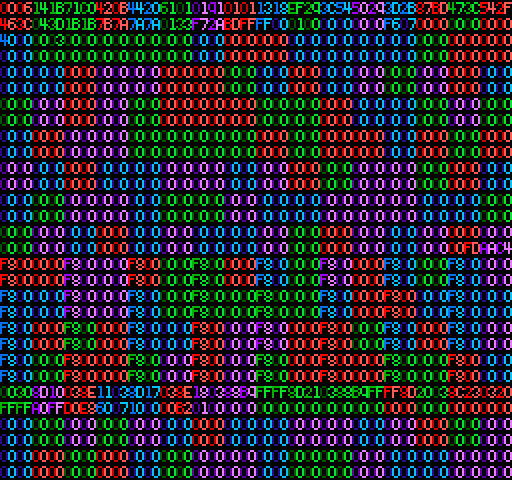
\includegraphics[width=0.9 \linewidth]{testrom}
  \caption{
    Exciting ``game''
  } \label{fig:testrom}
\end{figure}

Flinuint8

Goedelization?






% For posterity, old approaches to IsntZero
\begin{lstlisting}[language=C]
Fluint8 Fluint8::IsntZero(Fluint8 a) {
  // A simple way to do this is to extract all the (negated) bits
  // and multiply them together. But this would mean multiplying
  // a by itself, and so is not linear.
  //
  // Instead, do the same but ADD the bits. Now we have a
  // number in [0, 8]. So now we can do the whole thing again
  // and get a number in [0, 4], etc.

  half num_ones = (half)0.0f;
  Fluint8 aa = a;
  for (int bit_idx = 0; bit_idx < 8; bit_idx++) {
    Fluint8 aashift = RightShift1(aa);
    half a_bit = aa.h - LeftShift1Under128(aashift).h;
    num_ones += a_bit;
    aa = aashift;
  }

  ECHECK(num_ones >= (half)0.0f && num_ones <= (half)8.0f);

  // now count the ones in num_ones.
  aa = Fluint8(num_ones);
  num_ones = (half)0.0f;
  for (int bit_idx = 0; bit_idx < 4; bit_idx++) {
    Fluint8 aashift = RightShift1(aa);
    half a_bit = aa.h - LeftShift1Under128(aashift).h;
    num_ones += a_bit;
    aa = aashift;
  }

  ECHECK(num_ones >= (half)0.0f && num_ones <= (half)4.0f);

  // and again ...
  aa = Fluint8(num_ones);
  num_ones = (half)0.0f;
  for (int bit_idx = 0; bit_idx < 3; bit_idx++) {
    Fluint8 aashift = RightShift1(aa);
    half a_bit = aa.h - LeftShift1Under128(aashift).h;
    num_ones += a_bit;
    aa = aashift;
  }

  ECHECK(num_ones >= (half)0.0f && num_ones <= (half)3.0f);

  // and again ...
  aa = Fluint8(num_ones);
  num_ones = (half)0.0f;
  for (int bit_idx = 0; bit_idx < 2; bit_idx++) {
    Fluint8 aashift = RightShift1(aa);
    half a_bit = aa.h - LeftShift1Under128(aashift).h;
    num_ones += a_bit;
    aa = aashift;
  }

  ECHECK(num_ones >= (half)0.0f && num_ones <= (half)2.0f);

  // Now num_ones is either 0, 1, or 2. Since 1 and 2 is each
  // represented with a single bit, we can collapse them with
  // a shift and add:
  //   num_ones    output
  //         00         0
  //         01         1
  //         10         1
  Fluint8 nn(num_ones);
  return Fluint8(nn.h + RightShift1(nn).h);
}

static Fluint8 OldIsZero1(Fluint8 a) {
  // We know IsZero returns 1 or 0.
  // return Fluint8(1.0_h - IsntZero(a).h);

  Fluint8 aa = a;
  // true if everything is 1.0 so far
  half res = 1.0_h;
  for (int bit_idx = 0; bit_idx < 8; bit_idx++) {
    // leftmost bit
    half bit = RightShift<7>(aa).h;
    half nbit = (1.0_h - bit);
    // res = res & ~bit
    res = RightShiftHalf1(nbit + res);
    // aa = LeftShift<1>(aa);
    // We already have the high bit, so mask it off if necessary
    aa = Fluint8(aa.h - bit * 128.0_h);
    aa = LeftShift1Under128(aa);
  }

  return Fluint8(res);
}
\end{lstlisting}


% old approach to If

\begin{lstlisting}[language=C]
  // For cc = 0x01 or 0x00 (only), returns c ? t : 0.
Fluint8 Fluint8::If(Fluint8 cc, Fluint8 t) {
  // Multiplying cc * t gives us what we want, but this may
  // violate linearity (e.g.~if the two inputs are the same).

  // Could do this by spreading the cc to 0xFF or 0x00 (cc * 255 will
  // do that) and using AND, but it is faster to just keep consulting
  // the ones place of cc.

  half kept = GetHalf(0x0000);
  Fluint8 tt = t;
  for (int bit_idx = 0; bit_idx < 8; bit_idx++) {
    // Low order bit as a - ((a >> 1) << 1)
    Fluint8 ttshift = RightShift1(tt);
    half t_bit = tt.h - LeftShift1Under128(ttshift).h;
    // Computes 2^bit_idx
    const half scale = GetHalf(0x3c00 + 0x400 * bit_idx);

    const half and_bits = RightShiftHalf1(t_bit + cc.h);
    kept += scale * and_bits;

    // and keep shifting down
    tt = ttshift;
  }

  return Fluint8(kept);
}
\end{lstlisting}

\bibliography{grad}{}
\bibliographystyle{plain}

\end{document}
